\taskpic{ По внутренней поверхности большого неподвижного обруча
  радиусом $2r$ без проскальзывания катится малый обруч радиусом
  $r$. Отрезок $OO'$, соединяющий центры обручей, движется с угловой
  скоростью $\omega$. К малому обручу в точке $А$ прикреплён грузик. В
  некоторый момент времени обручи и грузик расположены так, как
  показано на рисунке. Чему равно в этот момент ускорение грузика?} 
{
  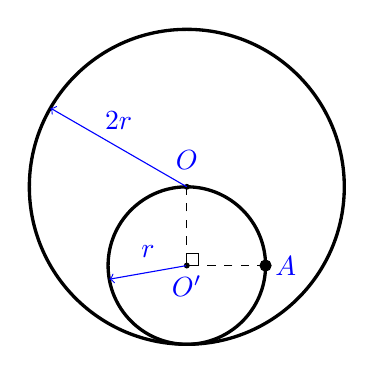
\begin{tikzpicture}
    \draw[very thick] (2,2) circle (2cm);
    \draw[very thick] (2,1) circle (1cm);
    \draw[fill=black] (2,2) circle (0.03cm); 
    \draw[fill=black] (2,1) circle (0.03cm); 
    \draw[blue,->] (2,2) node[above=0.1cm] {$O$} --++(150:2cm)
    node[above=0.1cm,midway] {$2r$};
    \draw[blue,->] (2,1) node[below] {$O'$} --++(190:1cm)
    node[above=0.07cm,midway] {$r$};
    \draw[dashed] (3,1) -- (2,1) -- (2,2);
    \draw[fill=black] (3,1) circle (0.07cm) node[right,blue] {$A$};
    \draw (2,1) rectangle ++(0.15,0.15);
  \end{tikzpicture}
}
% Московская городская олимпиада, 2006